% !Mode:: "TeX:UTF-8"
%% 请使用 XeLaTeX 编译本文.
\documentclass{HEBUTMaster}   % 选项 forprint: 交付打印时, 建议加上此选项, 以消除彩色链接文字, 避免彩色字迹打印偏淡.
                              % 选项 forlib: 提交给图书馆的电子版, 需要加上选项 forlib, 以消除空白页和彩色链接.
                              % 选项 smd: Specialist Master's Degree, 产生专业硕士学位论文封面、页眉.
%%%=== 参考文献=== %%%
\bibliographystyle{abbrv}        % 参考文献样式,  plain,unsrt,alpha,abbrv 等等
%%%%%%%%%%%%%%%%%%%%%%%%%%%%%%%%%%%%%%%%%%%%%%%%%%%%
\begin{document} 
%%%=====================================================================%%%
\title{混合可再生能源制氢系统的多目标优化问题}
\Etitle{Multi-objective optimization problem of hydrogen production system with hybrid renewable energy} % 英文题目
\author{程淑伟}
\StudentNumber{202032803115}   % 学号
\Eauthor{Chengshuwei}            %作者英文名
\Csupervisor{林涛\quad 教授}        %指导教师中文名、职称
\Esupervisor{Prof.~Lintao}     %指导教师英文名、职称
\Schoolname{School of Artificial Intelligence} %学院英文名. 不确定的话, 请看一下自己学院的网页上是怎么写的. 别搞错了!
\date{二〇二一年四月}                    % 硕士类只写年月. 要注意和英文日期一致!!
\Edate{Apr, 2020}                   % 英文封面日期

%%%=====================================================================%%%
\pdfbookmark[0]{封面}{title}         % 封面页加到 pdf 书签
\maketitle
%%%=====================================================================%%%
% !Mode:: "TeX:UTF-8"

%%% 此部分包含: (1) 英文封面 (无需改动) ; (2) 郑重声明 (无需改动).

%%%%%%%%%%%%%%%%%%%%%%%%%%%%%
%%% -------------  英文封面 (无需改动)-------------   %%%
%%%%%%%%%%%%%%%%%%%%%%%%%%%%%
\thispagestyle{empty}
\renewcommand{\baselinestretch}{1.5}  %下文的行距
\vspace*{0.5cm}

\begin{center}{\zihao{2} \the\Etitle \par}\end{center}

\vfill

\begin{center}
\zihao{4}
\begin{tabular}{ r l }
 Candidate:      &  {\sc \the\Eauthor}      \\
 Student Number: & {\the\StudentNumber} \\
 Supervisor:     &  {\sc \the\Esupervisor}   \\
 Major:          & \the\Emajor  \\
\ifsmd \else Speciality:     & \the\Especiality \fi
\end{tabular}

\vspace*{2cm}
\begin{center}
  \iflib % 向图书馆提交电子文档, 使用黑白校徽.
  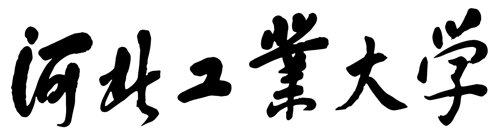
\includegraphics[height=4cm]{hebut.png}       %%  黑白的. 很小, 只有 10k.
  \else
     \ifprint % 文档打印, 使用黑白校徽.
  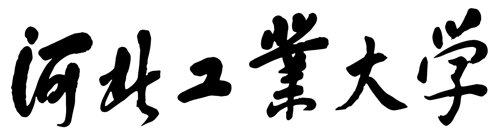
\includegraphics[height=4cm]{hebut.png}       %%  黑白的.
  \else
  
\includegraphics[height=4cm]{hebut1.png} %%  彩色的.
  \fi
  \fi
\end{center}


\zihao{-2}
\the\Schoolname\\
{\sc Hebei University of Technology}

\vspace*{1.0cm}

\the\Edate

\end{center}
%%%%%%%--判断是否需要空白页-----------------------------
 \iflib
 \else
\newpage
\thispagestyle{empty}
 \cleardoublepage
 \fi
%%%%%%%-------------------------------------------------
%%%--- 加入``郑重声明'' --- %%%%%%%%%%%%%%%%%
{\pagestyle{empty}
\newpage
\vspace*{20pt}
\begin{center}{\ziju{0.8}\zihao{-2}\heiti 论文原创性声明}\end{center}
\par\vspace*{30pt}
\renewcommand{\baselinestretch}{2}
{\zihao{4} \songti %


本人郑重声明: 所呈交的论文, 是本人独立进行研究工作所取得的研究成果.
除文中已经标明引用的内容外, 本论文不包含任何其他个人或集体已经发表或撰写过的研究成果.
对本文的研究做出贡献的个人和集体, 均已在文中以明确方式标明. 本声明的法律结果由本人承担.


\vskip2cm

\hspace*{4cm}学位论文作者(签名): \hspace{4cm} \hfill \\[1cm]
\hspace*{10cm}年 \hfill  月 \hfill 日\hspace{1cm}\hfill\par}

%%%%%%%--判断是否需要空白页-----------------------------
  \iflib
  \else
  \newpage
  \cleardoublepage
  \fi
%%%%%%%-------------------------------------------------
}
\renewcommand{\baselinestretch}{1.6}
\small\normalsize




    % 加入英文封面
\frontmatter
\pagenumbering{Roman}               % 正文之前的页码用大写罗马字母编号.

\cleardoublepage
\newpage  \pagestyle{fancy} \fancyfancy
%%%=====================================================================%%%
% !Mode:: "TeX:UTF-8"

%%% 说明: 此部分需要自己填写的内容:  (1) 中文摘要及关键词 (2) 英文摘要及关键词

%%%%%%%%%%%%%%%%%%%%%%%
%%% ------------ 中文摘要 ---------------%%%
%%%%%%%%%%%%%%%%%%%%%%%
\begin{cnabstract}


\end{cnabstract}
\vspace{1em}\par\vfill

%%%--------- 关键词 -------- %%%
\cnkeywords{}

%%%%%%%%%%%%%%%%%%%%%%%


%%%%%%%%%%%%%%%%%%%%%%%
%%% ------------ 英文摘要 ---------------%%%
%%%%%%%%%%%%%%%%%%%%%%%

\begin{enabstract}





\end{enabstract}
\vspace{1em}\par\vfill

%%%------ 英文关键词 ------- %%%
\enkeywords{}


      % 加入中英文 摘要 .
%---把目录加入到书签---%%%%%%%%%%%%%%
\pdfbookmark[0]{目录}{toc}%%%%%%%%%%%%

\tableofcontents
%%%=====================================================================%%%
\mainmatter %% 以下是正文
\baselineskip=20pt  % 正文行距为 20 磅
%%%=====================================================================%%%
\chapter{简介}

\section{研究背景}

\section{文献调查} 

\section{本文工作}

\section{文章结构}


%%%================================第二章=====================================%%%
\chapter{方法}
%%%================================第2.1章=====================================%%%
\section{系统建模}

\subsection{光电阵列}

\subsection{风机装置}

\subsection{制氢装置}

\subsection{锂电池组}

%%%================================第2.2章=====================================%%%
\section{目标优化}

\subsection{评估标准}

\subsection{约束模型}


%%%================================第三章=====================================%%%
\chapter{优化}
%%%================================第3.1章=====================================%%%

\section{传统优化}

\section{粒子群优化}

\section{多目标粒子群}

\subsection{提出算法}

\subsection{算法流程}

%%%================================第四章=====================================%%%
\chapter{结果}

%%%================================第五章=====================================%%%
\chapter{总结}

%%%================================第5.1章=====================================%%%



%%%=== 参考文献 ========%%%
\cleardoublepage\phantomsection
\addcontentsline{toc}{chapter}{参考文献}
\begin{thebibliography}{000}\zihao{5}

  \bibitem{r1}
  \bibitem{r2}
  \bibitem{r3}
  \bibitem{r4}
  \bibitem{r5}  
  \bibitem{r6}
  
\end{thebibliography}


\acknowledgement
感谢曹斌老师布置的作业, 加快了我科研的脚步,感谢!

%\backmatter
%% !Mode:: "TeX:UTF-8"

%%% 此部分内容:  (1) 致谢  (2) 河北工业大学学位论文使用授权协议书(无需改动)

%%%%%%%%%%%%%%%%%%%%%%%
%%% --------------- 致谢 ------------- - %%%
%%%%%%%%%%%%%%%%%%%%%%%
\acknowledgement


感谢你, 感谢他和她, 感谢大家.







%%%%%---河北工业大学学位论文使用授权协议书---%%%%%%%%%%%%
%%%%%%%%%%%%%%%%%%%%%%%%%%%%%%%%%%%
%%%%%%%%%%%%%%%%%%%%%%%%%%%%%%%%%%%
\cleardoublepage
\newpage\vspace*{20pt}
\begin{center}{\zihao{-2}\heiti 河北工业大学学位论文使用授权协议书}\end{center}
\par\vspace*{30pt}

本论文作者愿意遵守河北工业大学关于保存、使用学位论文的管理办法及规定,
即:学校有权保存学位论文的印刷本和电子版, 并提供文献检索与阅览服务;
学校可以采用影印、缩印、数字化或其它复制手段保存论文;
在以教学与科研服务为目的前提下, 学校可以在校园网内公布部分及全部内容.
\begin{enumerate}[1、]
  \item  在本论文提交当年, 同意在校园网内以及中国高等教育文献保障系
           统(CALIS)高校学位论文系统提供查询及前十六页浏览服务.
  \item  在本论文提交~$\Box$~当年/~$\Box$~一年/~$\Box$~两年
            /~$\Box$~三年/~$\Box$~五年以后, 同意在校园网内允许读者
            在线浏览并下载全文, 学校可以为存在馆际合作关系的兄弟高校用
            户提供文献传递服务和交换服务.(保密论文解密后遵守此规定)
\end{enumerate}

\vskip 15mm

论文作者(签名):\raisebox{-1ex}{\underline{\makebox[5cm][c]{}}}
\vskip2em
				          				
学\qquad\qquad\quad 号:\raisebox{-1ex}{\underline{\makebox[5cm][c]{}}}
\vskip2em	
					
学\qquad\qquad\quad 院:\raisebox{-1ex}{\underline{\makebox[5cm][c]{}}}					

\vskip  2cm
\begin{flushright}
 日期:\hskip2cm 年\hskip1.2cm 月\hskip1.2cm 日
\end{flushright}

%%%%%%%%%%%%%%%%%%%%%%%%%%%%%%%%%%%%%%%
%%%%%%%--判断是否需要空白页-----------------------------
  \iflib
  \else
  \newpage
 \cleardoublepage
  \fi
%%%%%%%-------------------------------------------------







 %%%致谢, 河北工业大学学位论文使用授权协议书.

\cleardoublepage

\end{document}



